% !TeX root = ../navier-stokes-manuscript.tex
% ============================================================
% 1.6 A Comparison with Euler
% ============================================================
\subsection{A Comparison with Euler}\label{sub:AComparisonWithEuler}

Let's run the thought experiment on one packet of fluid.
Draw an imaginary frame around it, with one horizontal line across the bottom of the packet and another across the top.
Those lines are not plates, walls, or the edges of a separate object.
They only let us keep track of the same fluid while we assign one tangential velocity, \(U_-e_1\), near the lower line and another, \(U_+e_1\), near the upper line, with \(U_-\neq U_+\).
We have fixed the two velocity readings without yet saying how the fluid between them behaves.

First imagine that the packet joins those readings continuously.
Every layer takes a velocity between \(U_-e_1\) and \(U_+e_1\), with neighbouring layers differing only slightly.
This is the velocity relation made familiar by Couette flow.
In the usual laboratory description, moving plates create and maintain the shear.
We are not putting those plates into the proposed fluid field here; we are borrowing the Couette profile and asking the packet itself to take on that smooth relation.

If the imaginary lines are separated by a distance \(h\), the profile inside the packet is
\[
  u_C(x)
  =
  \left(
    U_-+\frac{U_+-U_-}{h}x_3
  \right)e_1,
  \qquad
  0<x_3<h,
  \qquad
  p=p_0.
\]
Its velocity changes continuously from one sampled face to the other.
Its shear
\[
  \partial_3(u_C)_1
  =
  \frac{U_+-U_-}{h}
\]
is nonzero and finite throughout the packet.
There is no layer at which the velocity breaks away from the layers beside it.
\Cref{fig:CouetteFlow} draws the imaginary packet and the continuous family of intermediate speeds.

% !TeX root = ../../navier-stokes-manuscript.tex
\begin{figure}[!htbp]
  \centering
  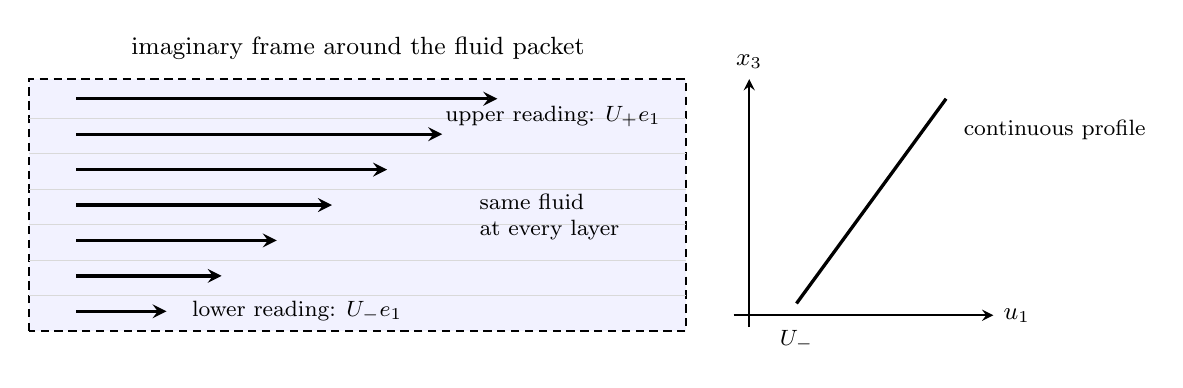
\begin{tikzpicture}[
    x=1cm,
    y=1cm,
    >=stealth,
    velocity/.style={->,very thick},
    smalllabel/.style={font=\small},
    tinylabel/.style={font=\footnotesize}
  ]
    \fill[blue!5]
      (0.50,0.65) rectangle (8.85,3.85);
    \draw[densely dashed,thick]
      (0.50,0.65) rectangle (8.85,3.85);

    \foreach \y in {1.10,1.55,2.00,2.45,2.90,3.35}
      \draw[black!15] (0.50,\y) -- (8.85,\y);

    \draw[velocity] (1.10,0.90) -- (2.25,0.90);
    \draw[velocity] (1.10,1.35) -- (2.95,1.35);
    \draw[velocity] (1.10,1.80) -- (3.65,1.80);
    \draw[velocity] (1.10,2.25) -- (4.35,2.25);
    \draw[velocity] (1.10,2.70) -- (5.05,2.70);
    \draw[velocity] (1.10,3.15) -- (5.75,3.15);
    \draw[velocity] (1.10,3.60) -- (6.45,3.60);

    \node[tinylabel,anchor=east] at (8.65,3.38)
      {upper reading: \(U_+e_1\)};
    \node[tinylabel,anchor=west] at (2.45,0.90)
      {lower reading: \(U_-e_1\)};
    \node[smalllabel,anchor=south] at (4.68,3.98)
      {imaginary frame around the fluid packet};
    \node[tinylabel,align=left,anchor=west] at (6.10,2.10)
      {same fluid\\at every layer};

    \draw[->,thick] (9.65,0.70) -- (9.65,3.85)
      node[above,smalllabel] {\(x_3\)};
    \draw[->,thick] (9.45,0.85) -- (12.75,0.85)
      node[right,smalllabel] {\(u_1\)};
    \draw[very thick] (10.25,1.00) -- (12.15,3.60);
    \node[tinylabel,anchor=north] at (10.25,0.78) {\(U_-\)};
    \node[tinylabel,anchor=west] at (12.25,3.20)
      {continuous profile};
  \end{tikzpicture}
  \caption{Continuous shear imagined inside one fluid packet.
  The dashed outline is only an observation frame.
  Every layer takes an intermediate velocity, so the one velocity field remains smooth across the packet.}
  \label{fig:CouetteFlow}
\end{figure}


The picture is smooth, but the equations still have to classify it.
Because the velocity points in the \(e_1\)-direction and varies only in the \(x_3\)-direction,
\[
  \nabla\cdot u_C=0,
  \qquad
  (u_C\cdot\nabla)u_C=0,
  \qquad
  \Delta u_C=0,
  \qquad
  \nabla p=0.
\]
The profile satisfies the local Euler momentum law and the local fixed-viscosity \NavierStokes{} momentum law at the same time.
It lies in the overlap of the two local equation classes.
Positive viscosity is present in the \NavierStokes{} law, but this linear profile has no spatial curvature for the Laplacian to act on.
The nonzero shear therefore does not become a nonzero bulk viscous force.

Now keep the same packet, the same imaginary frame, and the same two velocity readings.
Change only the way the fluid joins them.
Imagine all the fluid below a middle plane moving with \(U_-e_1\) and all the fluid above it moving with \(U_+e_1\), with no intermediate velocities between them.
The fluid is being asked to move in a board-like way, but there are no boards and there are not two bodies.
It is still one fluid packet, now carrying an abrupt tangential jump across an internal surface.
\Cref{fig:BoardLikeSlip} draws that second imagined behaviour inside the same kind of packet.

% !TeX root = ../../navier-stokes-manuscript.tex
\begin{figure}[!htbp]
  \centering
  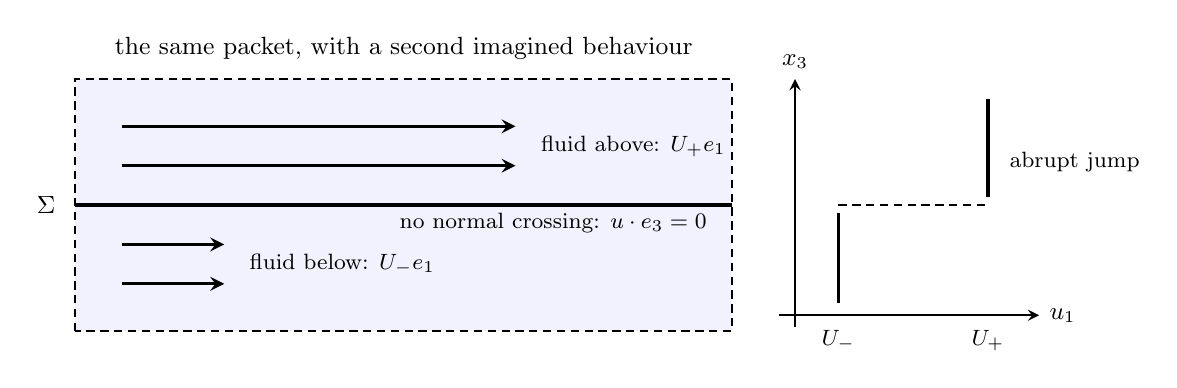
\begin{tikzpicture}[
    x=1cm,
    y=1cm,
    >=stealth,
    velocity/.style={->,very thick},
    smalllabel/.style={font=\small},
    tinylabel/.style={font=\footnotesize}
  ]
    \fill[blue!5]
      (0.50,0.65) rectangle (8.85,3.85);
    \draw[densely dashed,thick]
      (0.50,0.65) rectangle (8.85,3.85);
    \draw[very thick] (0.50,2.25) -- (8.85,2.25);
    \node[smalllabel,anchor=east] at (0.38,2.25) {\(\Sigma\)};

    \draw[velocity] (1.10,1.25) -- (2.40,1.25);
    \draw[velocity] (1.10,1.75) -- (2.40,1.75);
    \draw[velocity] (1.10,2.75) -- (6.10,2.75);
    \draw[velocity] (1.10,3.25) -- (6.10,3.25);

    \node[tinylabel,anchor=west] at (6.30,3.00)
      {fluid above: \(U_+e_1\)};
    \node[tinylabel,anchor=west] at (2.60,1.50)
      {fluid below: \(U_-e_1\)};
    \node[smalllabel,anchor=south] at (4.68,3.98)
      {the same packet, with a second imagined behaviour};
    \node[tinylabel,anchor=east] at (8.65,2.02)
      {no normal crossing: \(u\cdot e_3=0\)};

    \draw[->,thick] (9.65,0.70) -- (9.65,3.85)
      node[above,smalllabel] {\(x_3\)};
    \draw[->,thick] (9.45,0.85) -- (12.75,0.85)
      node[right,smalllabel] {\(u_1\)};
    \draw[very thick] (10.20,1.00) -- (10.20,2.15);
    \draw[very thick] (12.10,2.35) -- (12.10,3.60);
    \draw[densely dashed] (10.20,2.25) -- (12.10,2.25);
    \node[tinylabel,anchor=north] at (10.20,0.78) {\(U_-\)};
    \node[tinylabel,anchor=north] at (12.10,0.78) {\(U_+\)};
    \node[tinylabel,anchor=west] at (12.25,2.80)
      {abrupt jump};
  \end{tikzpicture}
  \caption{Board-like motion imagined inside the same fluid packet.
  The dashed outline is not a wall, and the two regions are not separate bodies.
  The one velocity field jumps tangentially across \(\Sigma\), so this profile is nonsmooth even though its normal flow remains zero.}
  \label{fig:BoardLikeSlip}
\end{figure}


That jump is visibly nonsmooth, but its equation class cannot be decided by appearance alone.
We hold the proposed field fixed while Euler and \NavierStokes{} test the same velocity, pressure, incompressibility, and nonlinear momentum transport.
Written in divergence form, which remains meaningful across a jump, the local laws are
\[
  \begin{aligned}
  \text{Euler:}\qquad
  &\partial_tu+\nabla\cdot(u\otimes u)+\nabla p=0,\\
  \text{\NavierStokes:}\qquad
  &\partial_tu+\nabla\cdot(u\otimes u)+\nabla p=\nu\Delta u,
  \qquad \nu>0,
  \end{aligned}
\]
with \(\nabla\cdot u=0\) in both cases.
Both laws test the velocity and its time change, nonlinear momentum transport, pressure, and incompressibility.
\NavierStokes{} adds the response to spatial curvature through \(\nu\Delta u\).
The common requirements come first; viscosity can separate the laws only after the proposed field passes them.

Let the internal interface be \(\Sigma=\{x_3=0\}\), with normal direction \(e_3\), and choose the same two tangential speeds \(U_-\) and \(U_+\).
The imagined field is
\[
  u(x)=
  \begin{cases}
    U_-e_1, & x_3<0,\\
    U_+e_1, & x_3>0,
  \end{cases}
  \qquad
  p(x)=p_0.
\]
Its jump is
\[
  [u]=(U_+-U_-)e_1,
\]
which lies entirely along the interface.
Write \(\delta_\Sigma\) for unit surface mass concentrated on \(\Sigma\).
The only possible divergence defect is the normal part of the jump, and here
\[
  \nabla\cdot u
  =
  [u]\cdot e_3\,\delta_\Sigma
  =
  (U_+-U_-)(e_1\cdot e_3)\,\delta_\Sigma
  =0.
\]
The fluid on the two sides slides tangentially without creating a source, a sink, or any mass flux through the plane.

The nonlinear transport has the same geometry.
On either side of \(\Sigma\),
\[
  (u\otimes u)e_3
  =
  u(u\cdot e_3)
  =0.
\]
Consequently there is no jump in normal momentum flux and \(\nabla\cdot(u\otimes u)=0\) as a distribution.
The field is stationary, so \(\partial_tu=0\), and the constant pressure contributes no force.
Every shared term in the Euler momentum law vanishes.

This stationary tangential discontinuity is called a planar vortex sheet.
It is a local distributional weak solution of the incompressible Euler equations.
Its velocity is finite on both sides, while its shear is concentrated on the interface:
\[
  \nabla\times u
  =
  (U_+-U_-)e_2\,\delta_\Sigma.
\]
So Euler really does admit this imagined board-like behaviour of one fluid in the local model.

Now require fixed positive viscosity without changing any part of the stationary field.
The first derivative of the velocity is concentrated on \(\Sigma\), and the second derivative gives
\[
  \Delta u
  =
  (U_+-U_-)e_1\,\partial_3\delta_\Sigma.
\]
The left side of the stationary momentum equation is still zero, while \(\nu\Delta u\) is not.
Changing the pressure cannot supply the missing term.
Indeed,
\[
  \nabla\times(\nu\Delta u)
  =
  \nu(U_+-U_-)e_2\,\partial_3^2\delta_\Sigma
  \neq0,
  \qquad
  \nabla\times\nabla p=0
\]
for every scalar pressure distribution \(p\).
The same velocity -- pressure candidate passes the local Euler law and fails the fixed-viscosity \NavierStokes{} momentum law.
The two imagined behaviours can now be classified without changing the packet under discussion.
The continuous Couette-like profile is smooth and lies in the local overlap of Euler and \NavierStokes{}.
The abrupt profile is nonsmooth, lies in the local Euler class, and lies outside the local fixed-positive-viscosity \NavierStokes{} class.

The static failure also says what a viscous evolution does in place of the stationary jump.
Keep the same planar geometry and allow its tangential speed to change in time:
\[
  u(t,x)=(U(t,x_3),0,0),
  \qquad
  p=p_0.
\]
Incompressibility is automatic, and nonlinear transport vanishes because the velocity points in the \(x_1\)-direction while the profile varies only in \(x_3\).
The two equations reduce to
\[
  \text{Euler:}\quad \partial_tU=0,
  \qquad
  \text{\NavierStokes:}\quad \partial_tU=\nu\partial_3^2U.
\]
Euler leaves every such tangential profile fixed in this planar ansatz.
\NavierStokes{} turns the same profile into one-dimensional heat flow.
Starting from the two assigned packet speeds,
\[
  U(0,x_3)=
  \begin{cases}
    U_-, & x_3<0,\\
    U_+, & x_3>0,
  \end{cases}
\]
the viscous profile at every \(t>0\) is
\[
  U(t,x_3)
  =
  \frac{U_-+U_+}{2}
  +
  \frac{U_+-U_-}{2}
  \operatorname{erf}\!\left(\frac{x_3}{2\sqrt{\nu t}}\right).
\]
The sharp interface disappears immediately, and most of the change is spread through a layer whose thickness is comparable to \(\sqrt{\nu t}\).
Euler preserves the slip; positive viscosity communicates tangential momentum across it and rounds it into a smooth transition.

This also completes the comparison with the smooth packet.
The Couette-like profile has \(\partial_3^2u_1=0\) throughout the imagined packet, so it produces no viscous bulk residual there.
The step has a distributional second derivative at its internal interface, so the fixed-positive-viscosity evolution cannot keep that step stationary.
Physical plates maintain the shear in a laboratory Couette experiment, but the lines drawn around the packet in either picture never supplied that forcing and never became part of the fluid field.

The calculation separates the local governing laws, while full class membership asks for more.
The infinite sheet does not decay, has infinite kinetic energy on \(\mathbb R^3\), lies outside \(H^1\), and is unrelated to the fixed datum and preterminal history in \cref{sub:ClassMembershipAndParticipation}.
It is neither a whole-space Millennium counterexample nor a full member of that continuation class.

Even if those global defects were set aside and the stationary sheet were offered as a proposed continuation \(Q\), its unmatched viscous distribution alone would force
\[
  \neg\operatorname{Member}(Q).
\]
The sheet still satisfies the Euler requirements we actually tested: pressure, incompressibility, and momentum balance.
The same stationary field fails when fixed positive viscosity is required by the \NavierStokes{} equation.

Here the loss of smoothness occurs in the velocity itself, so the separation is visible as soon as the two sides move at different speeds.
A subtler field may keep its velocity finite and continuous while its gradient, material acceleration, jerk, or some higher mixed derivative loses finite control.
The board-like jump exposes the lowest rung; the same class question remains when the first disagreement is hidden higher in the response of the fluid.
